\section{Evaluation}
This section presents the experimental results for Ostrich on an Intel 32-cores multicore machine. 
We mainly compare the performance of \myds with Phoenix.

We evaluate \myds and Phoenix on a 32-core Intel 4× Xeon E7-4820 system equipped with 128GB of RAM. 
The operating system is Ubuntu 12.04 with kernel 3.2.0 and glibc-2.15.
Benchmarks were built as 64-bit executables with gcc -O3.
We logically disable CPU cores using Linux’s CPU hotplug mechanism, which allows to disable or enable individual CPU cores by writing “0” (or “1”) to a special pseudo file (/sys/devices/system/cpu/cpuN/online), and the total number of threads was matched to the number of CPU cores enabled.
Each workload is executed 10 times. 
To reduce the effect of outliers, the lowest and the highest runtimes for each workload are discarded, and thus each result is the average of the remaining 8 runs.

%\subsection{ Performance Improvements Summary}
%\subsection{Benckmarks}
\subsection{Performance and Scalability}
%描述benchmarks的特点,benchmarks的数据集等
In this subsection, we measured the performance and scalability of \myds, and compare it with Phoenix.  
Since there are many heap objects shared among threads in Phoenix, and it is sensitive to memory allocator.
The memory allocator in glibc (i.e. ptmalloc\cite{gloger1997ptmalloc}), does not scale on multicore system. 
Compared to ptmalloc\cite{gloger1997ptmalloc}, jemalloc provided improved performance and scalability\cite{evans2006jemalloc}. 
Therefore, we evaluate performance and scalability of Phoenix with jemalloc and ptmalloc, respectively.

\subsubsection{Performance}
Based on \myth, we implemented the optimization of Phoenix in Section 4 and measured \myds performance by executing each benchmark, including histogram (\codet{hist}), linear\_regression (\codet{lr}), string\_match (\codet{sm}), wordcount (\codet{wc}), and pca. \redt{Why use these benchmark?}
Table II describes the workloads and their input datasets. 
\begin{figure}[!h!t]  
	\centering
	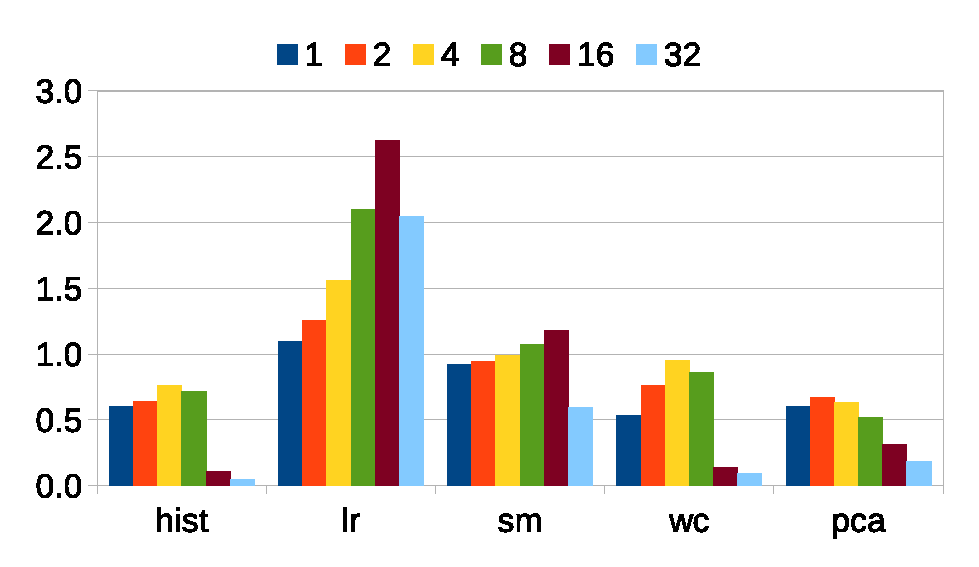
\includegraphics[width=0.45\textwidth]{eps/dmr_time_array.eps}
	\caption{SMR versus Phoenix with ptmalloc}
	\label{fig:smr:time:ptmalloc}
\end{figure}

Figure\ref{fig:smr:time:ptmalloc} measures the relative speedup of \myds over Phoenix-ptmalloc. 
As shown in the Figure \ref{fig:smr:time:ptmalloc}, For \codet{hist}, \code{wc} and \code{pca}, the optimized runtime of \myds leads to improvements across all core counts.
For less then 8 cores, the average improvement was \redt{2.0x} and the variation across applications were rather small.
For more then 8 cores, specially with 16 and 32 cores, the improvement were obvious, reaching \redt{10.x} in maximum and \redt{5.0x} on average.
For sm, it has performed as well as Phoenix when the cores number less then 16, while it better than Phoenix when there is more cores.
However, \myds runs worse than Phoenix on \code{lr} (about 0.8x).
\begin{figure}[!h!t]  
	\centering
	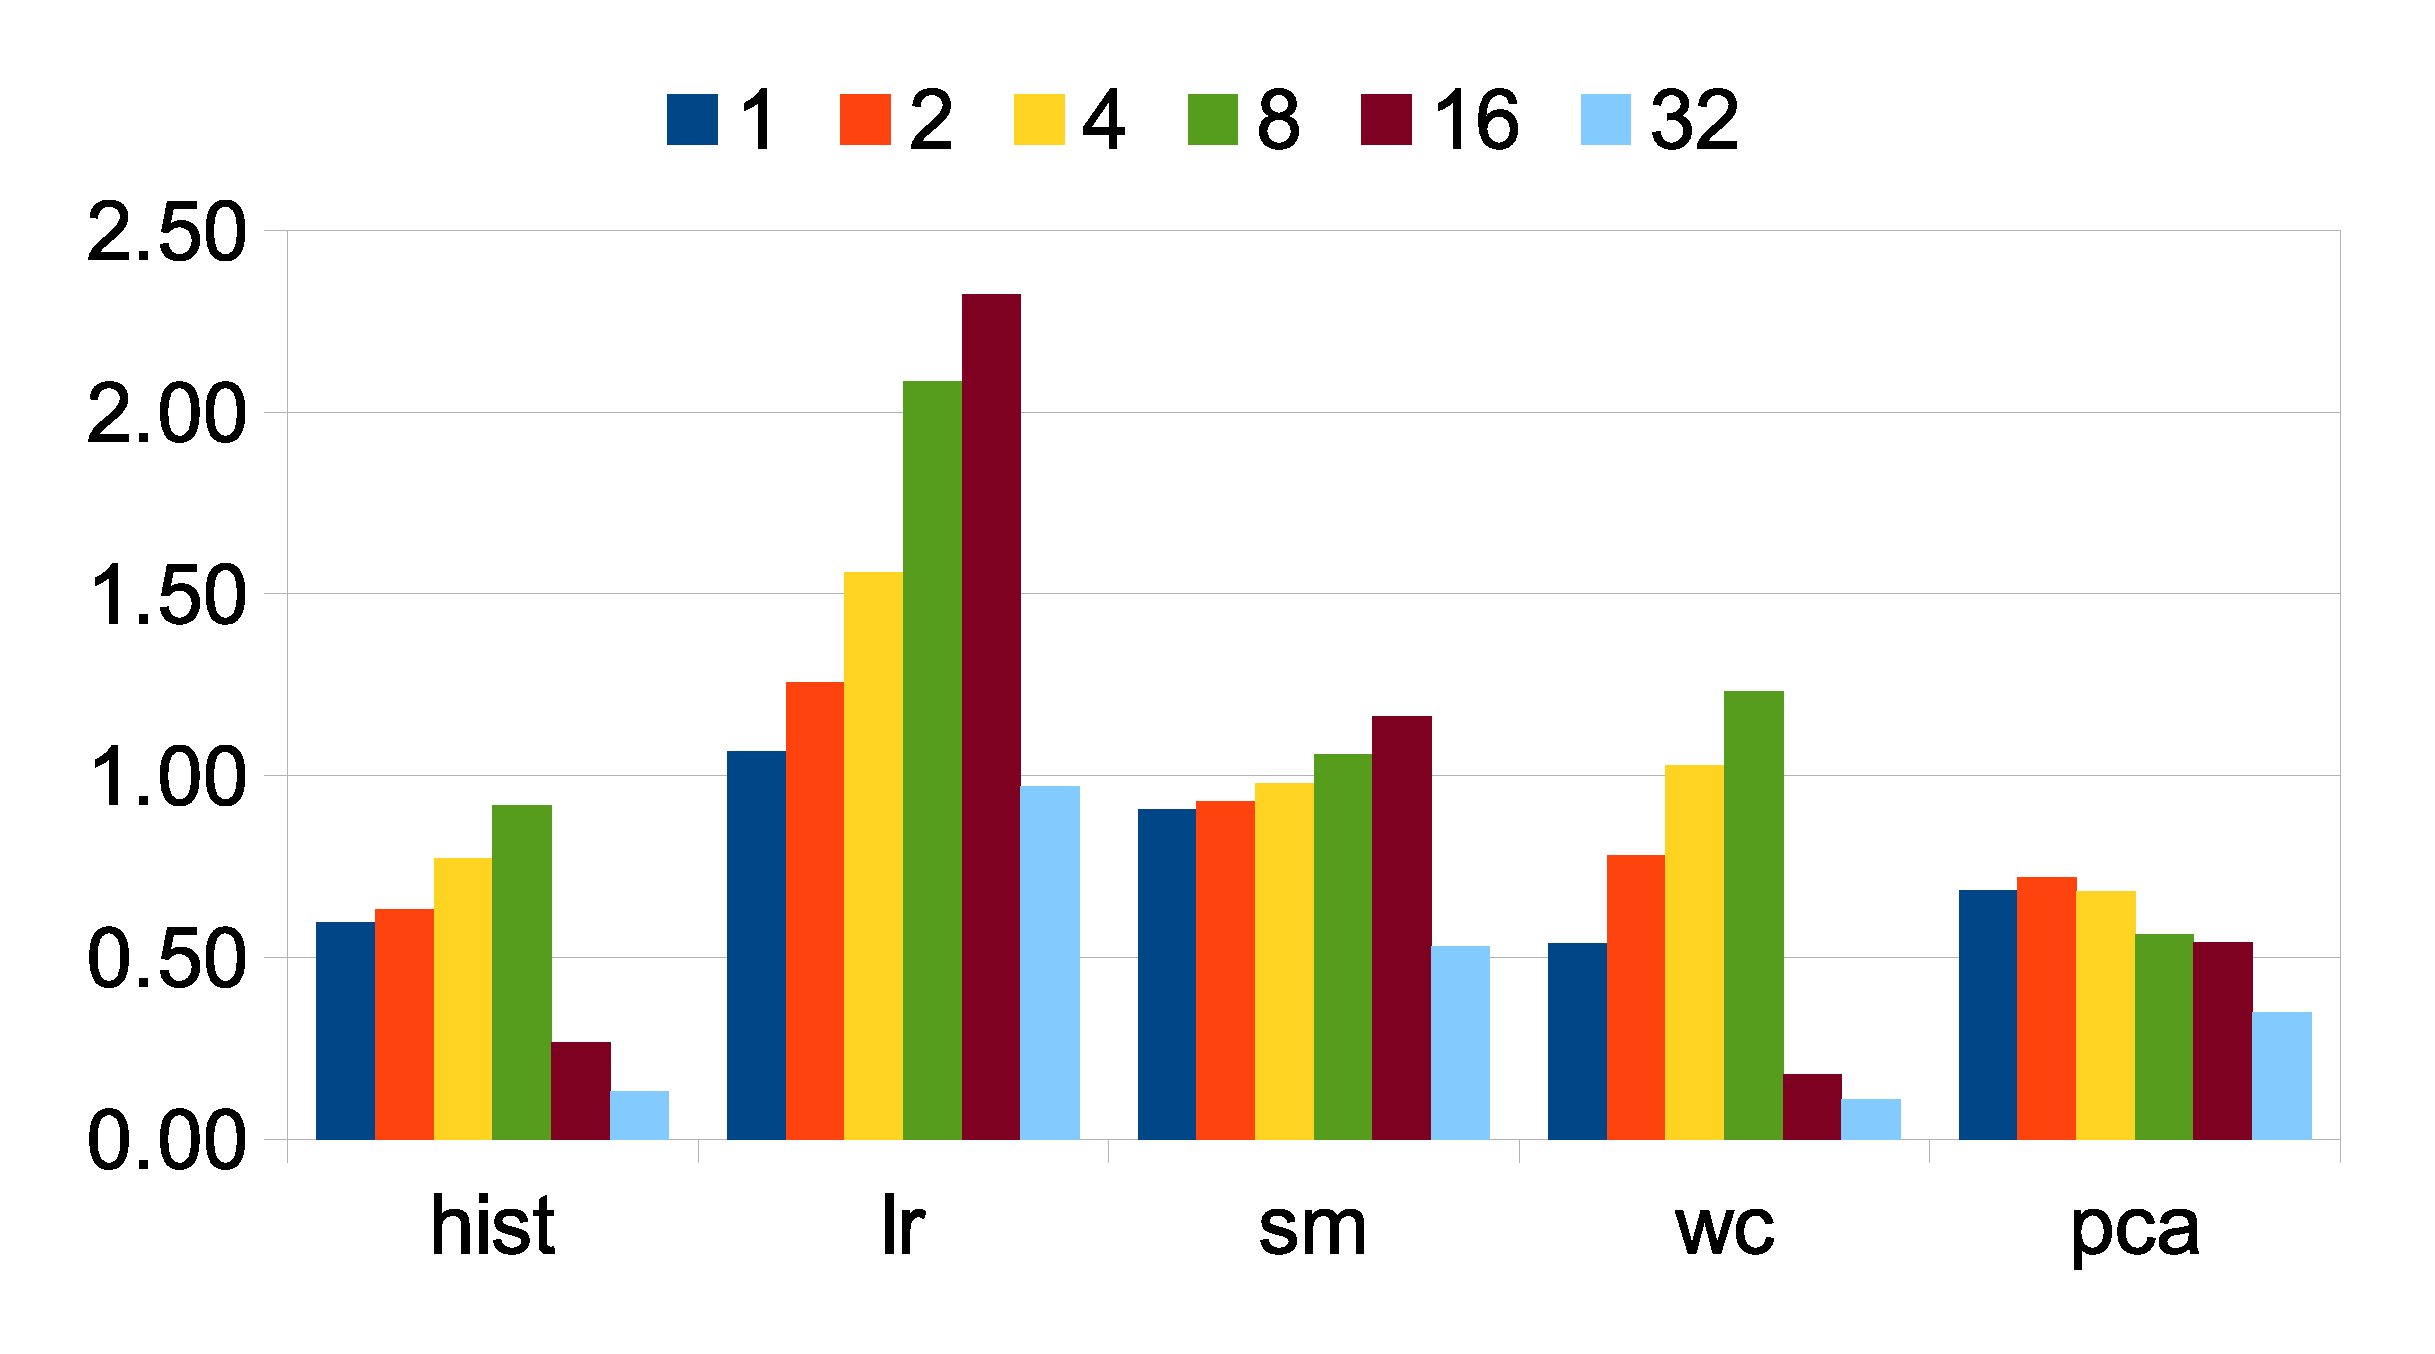
\includegraphics[width=0.45\textwidth]{eps/dmr_time_jemalloc.eps}
	\caption{SMR versus Phoenix with jemalloc}
	\label{fig:smr:time:jemalloc}
\end{figure}

Figure\ref{fig:smr:time:jemalloc} measures the relative speedup of \myds over Phoenix-jemalloc. 
We saw similar tendency when compared with Phoenix-jemalloc in Figure\ref{fig:smr:time:jemalloc}, while Phoenix with jemalloc has a better performacne.
Compared to Phoenix, we significantly increased the performance.
However, workloads, such as \code{lr} and \code{sm}, still did not scale particularly well. 
The reason of worse performance on linear\_regression is that most of time is waste in \myds's initailization.
We will evaluation overhead of initialization time in Section 5.4.
We discuss their bottlenecks in detail in Section 5.4, but in the remainder of this section we first focus on the optimizations that turned out to be successful.
\redt{need to explain why hist, wc, pca has good performance}

%\begin{figure}[htpb]
%	\centering
%	\subfigure[SMR versus Phoenix with ptmalloc]{
%		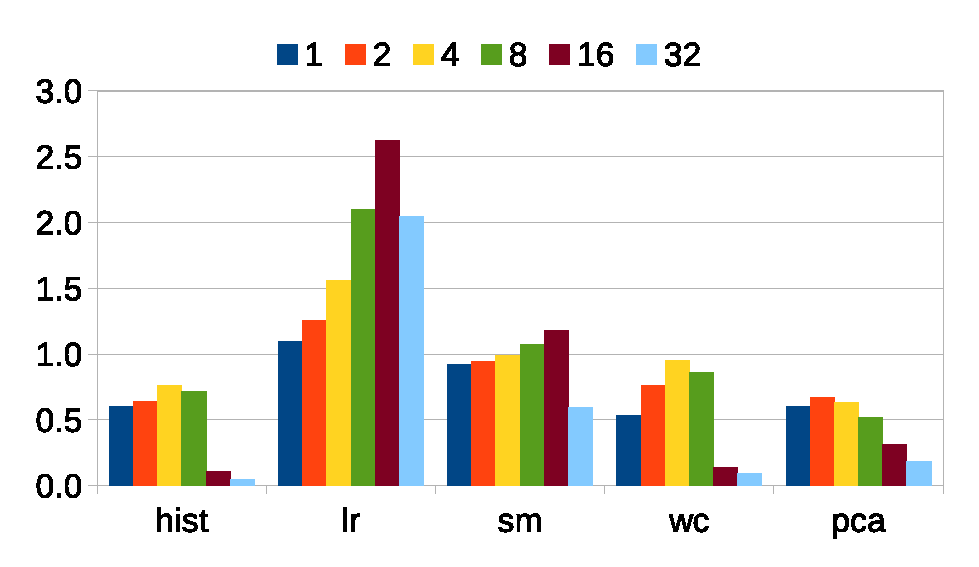
\includegraphics[width=0.45\textwidth]{eps/dmr_time_array.eps}
%		\label{fig:smr:time:ptmalloc}
%	}
%	\subfigure[SMR versus Phoenix with jemalloc]{
%		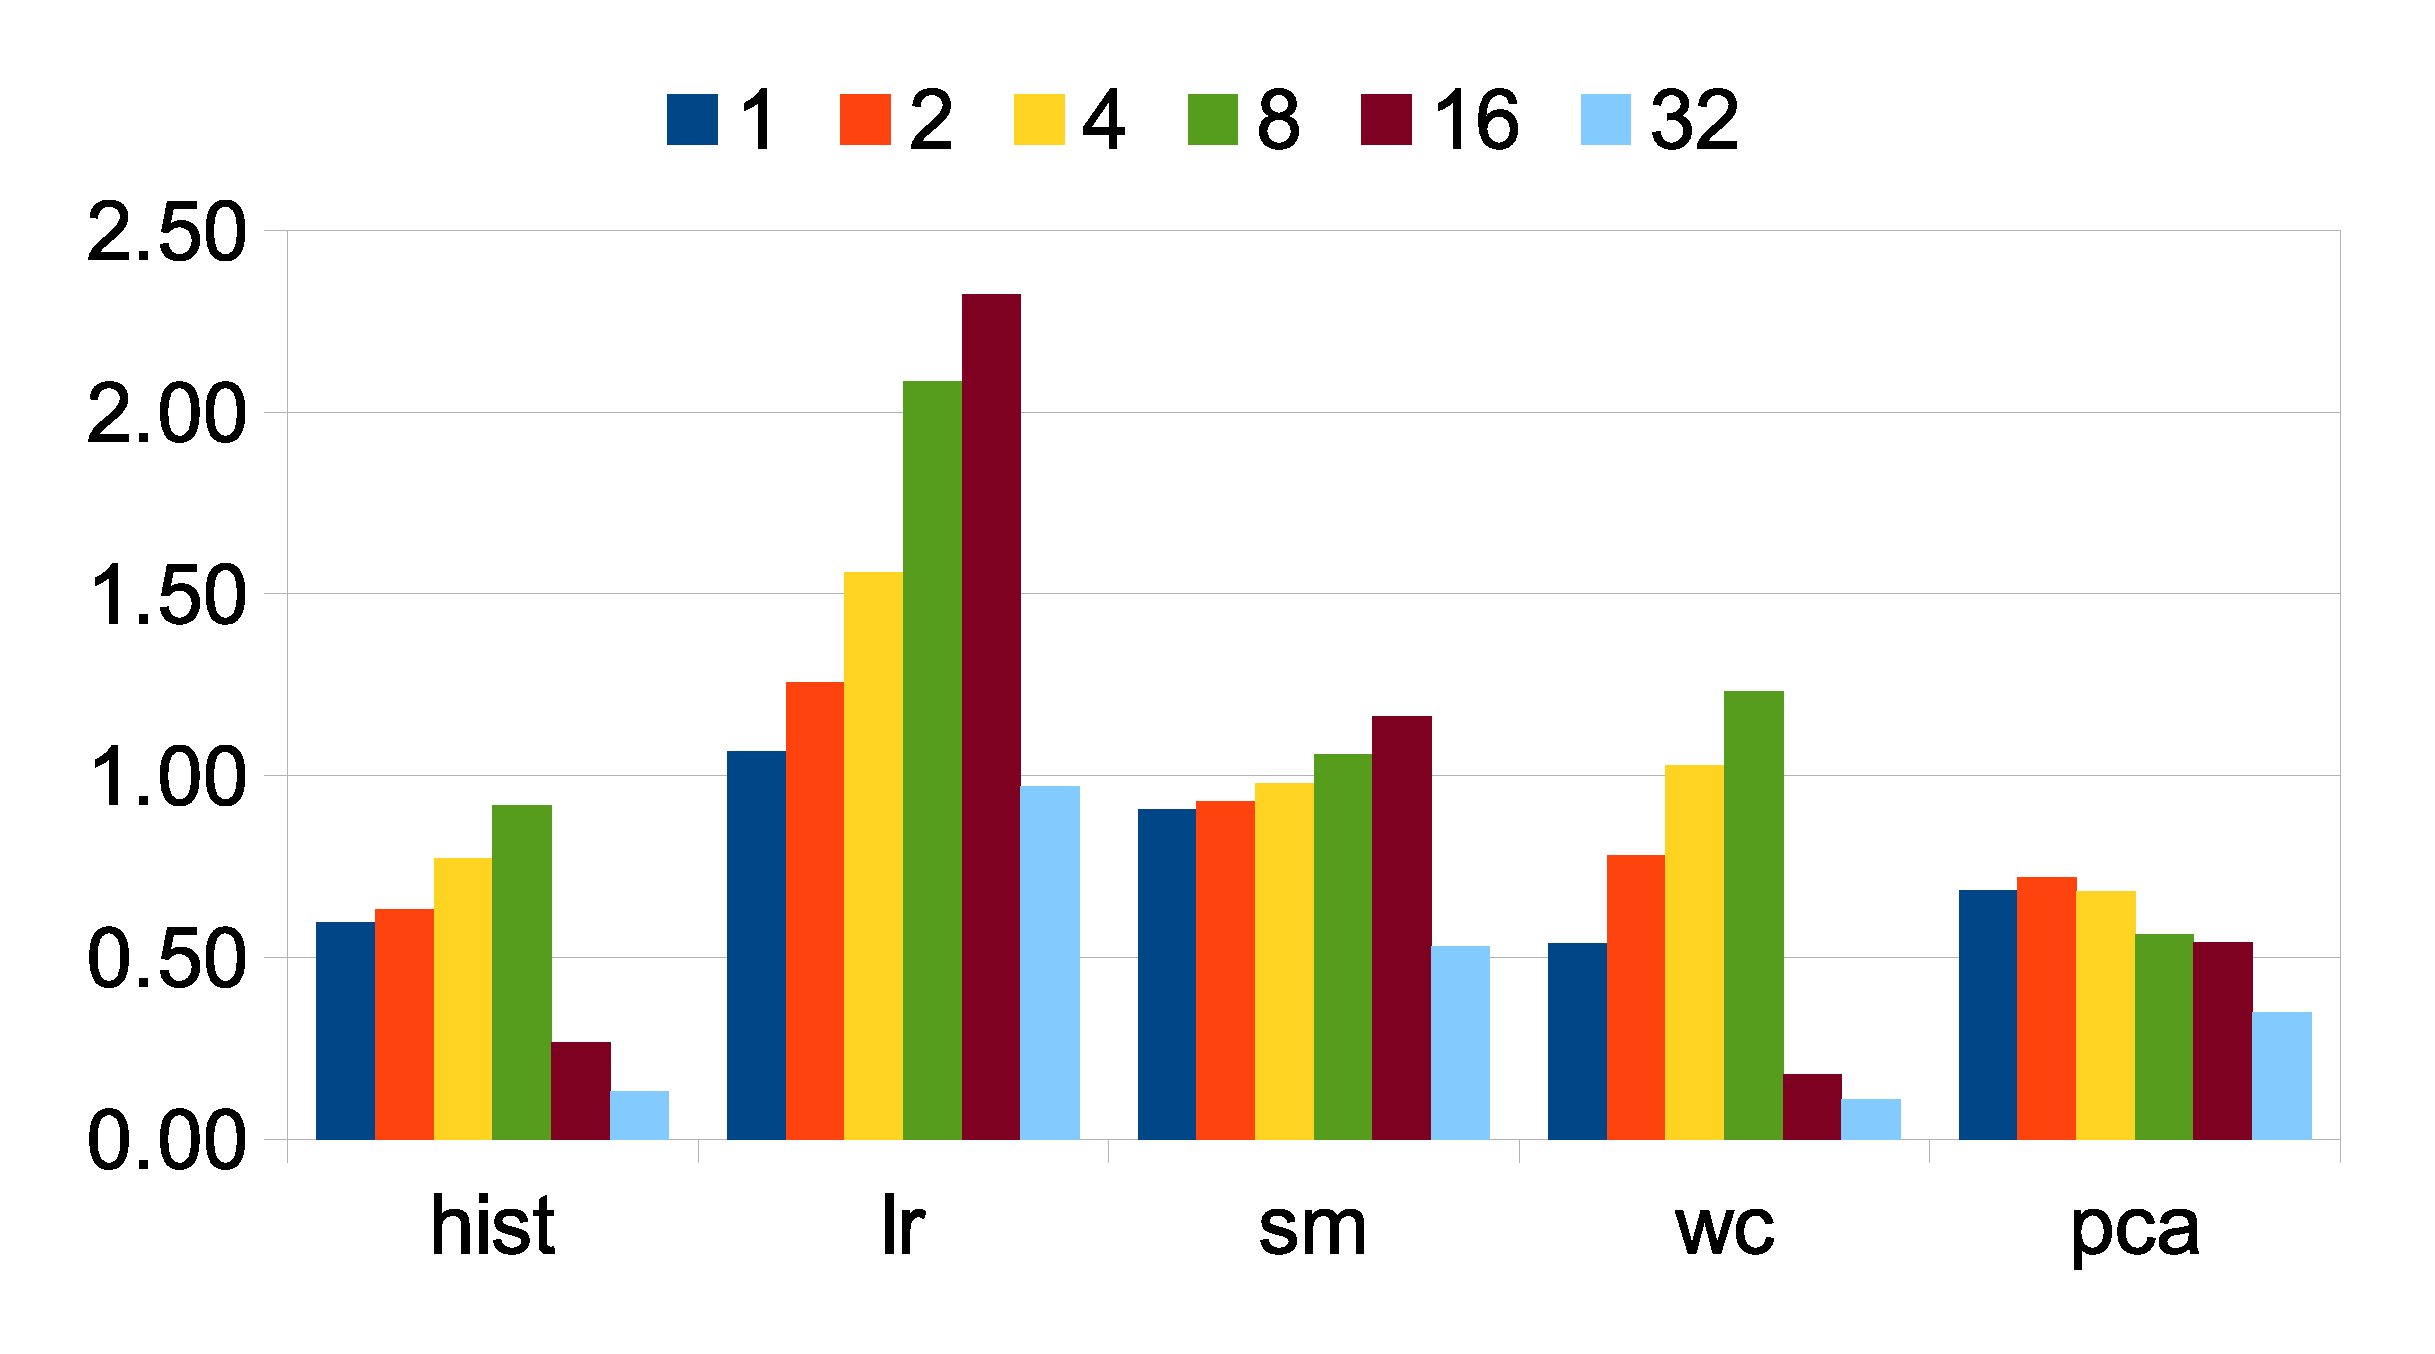
\includegraphics[width=0.45\textwidth]{eps/dmr_time_jemalloc.eps}
%		\label{fig:smr:time:jemalloc}
%	}
%	\caption{Execution time of SMR versus Phoenix}
%	\label{fig:time}
%\end{figure}


%However, nether allocator could successfully scaled up to 32cores.
%
%Figure\ref{fig:dmr:time:ptmalloc} and \ref{fig:dmr:time:jemalloc}
%present the Execution time of \myds versus Phoenix.
%%虽然jemalloc的性能表现要比ptmalloc好,但实验结果都显示
%\myds matches or outperforms Phoenix on 4 out of 5 workloads,
%but runs worse than Phoenix only on linear\_regression.
%For hist, pca and word\_count, 
%\myds outperforms Phoenix betwen xxx and xxx faster.

%从实验的结果可以看出,hist, wc, pca,SMR的性能较好,sm相当,lr中SMR的性能表现较差



%\begin{figure*}[htpb]
%\centering
%  \subfigure[]{
%   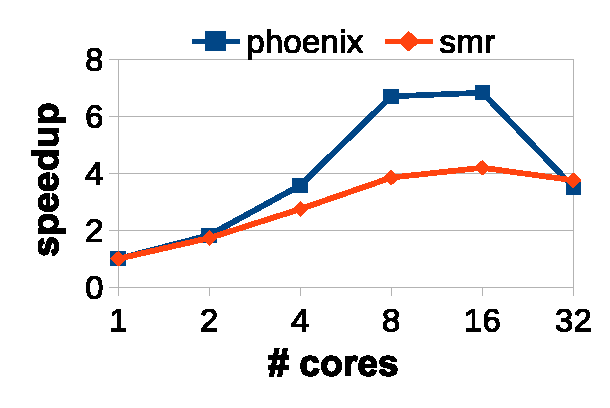
\includegraphics[width=0.15\textwidth]{eps/smr_scala_hist.eps}
%   \label{fig:dmr:time:ptmalloc}
%   }
%  \subfigure[]{
%	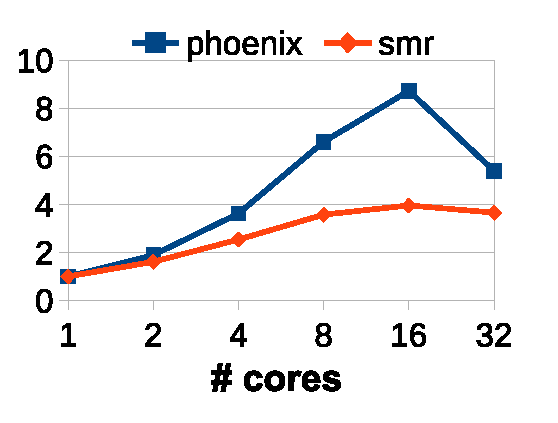
\includegraphics[width=0.15\textwidth]{eps/smr_scala_lr.eps}
%	\label{fig:dmr:time:ptmalloc}
%}
%  \subfigure[]{
%	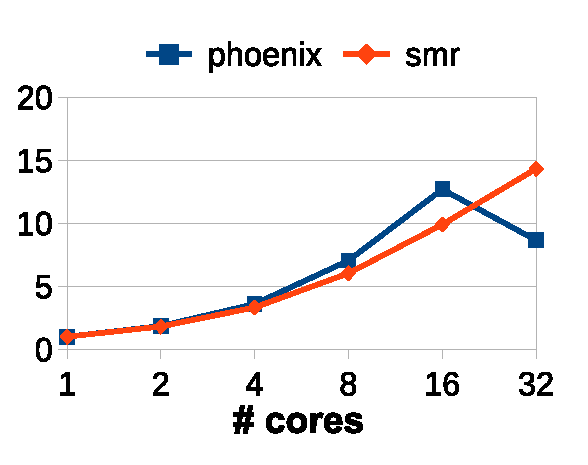
\includegraphics[width=0.15\textwidth]{eps/smr_scala_sm.eps}
%	\label{fig:dmr:time:ptmalloc}
%}
%  \subfigure[]{
%	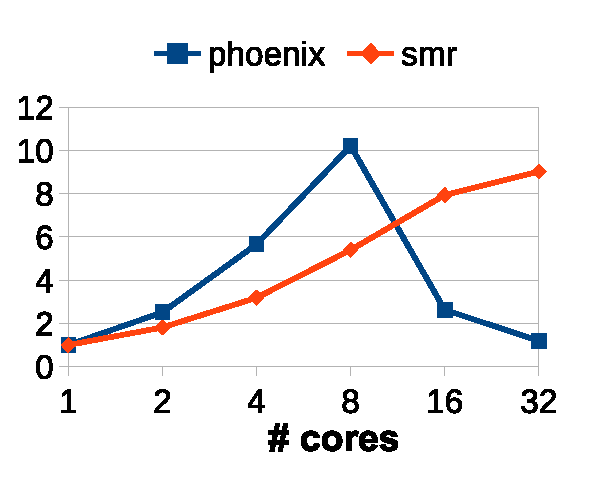
\includegraphics[width=0.15\textwidth]{eps/smr_scala_wc.eps}
%	\label{fig:dmr:time:ptmalloc}
%}
%  \subfigure[]{
%	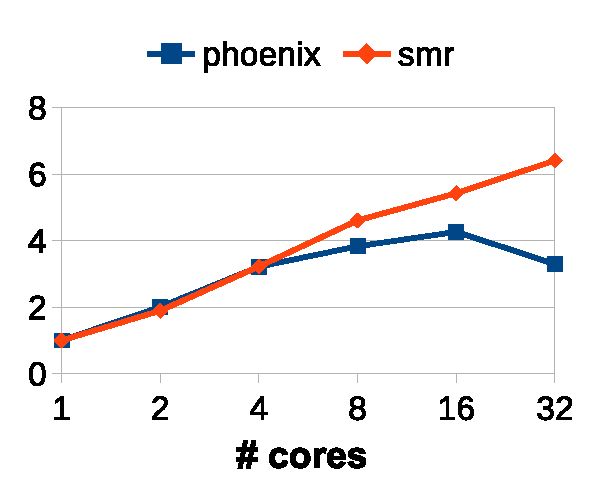
\includegraphics[width=0.15\textwidth]{eps/smr_scala_pca.eps}
%	\label{fig:dmr:time:ptmalloc}
%}
%  \caption{A comparison of the scalability of \myds with that of Phoenix}
%   \label{fig:scalability}
%\end{figure*}

\subsubsection{Scalability}
%Phoenix-jemalloc版本scalability存在的问题
\begin{figure}[!h!t]  
	\centering
	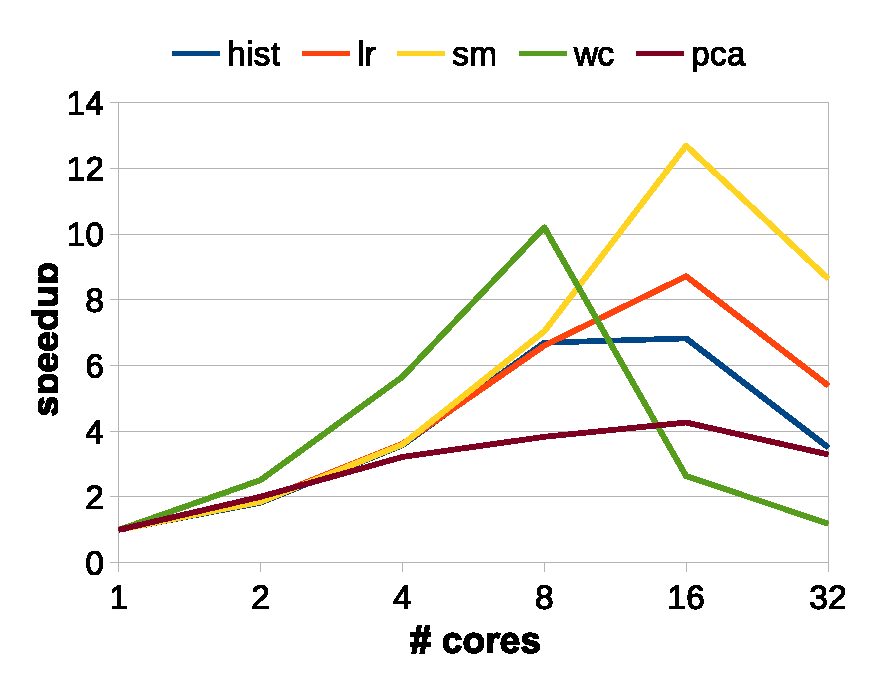
\includegraphics[width=0.45\textwidth]{eps/phoenix_speedup_jemalloc.eps}
	\caption{speedup of Phoenix-jemalloc}
	\label{fig:phoenix:speedup:jemalloc}
\end{figure}
Since Phoenix is sensitive to memory allocator, we evaluate its scalability with jemalloc, good scalability allocator.
Figure\ref{fig:phoenix:speedup:jemalloc} shows the speedup of Phoenix with jemalloc.
%\begin{figure}[htpb]
%	\centering
%	\subfigure[speedup of Phoenix-jemalloc]{
%		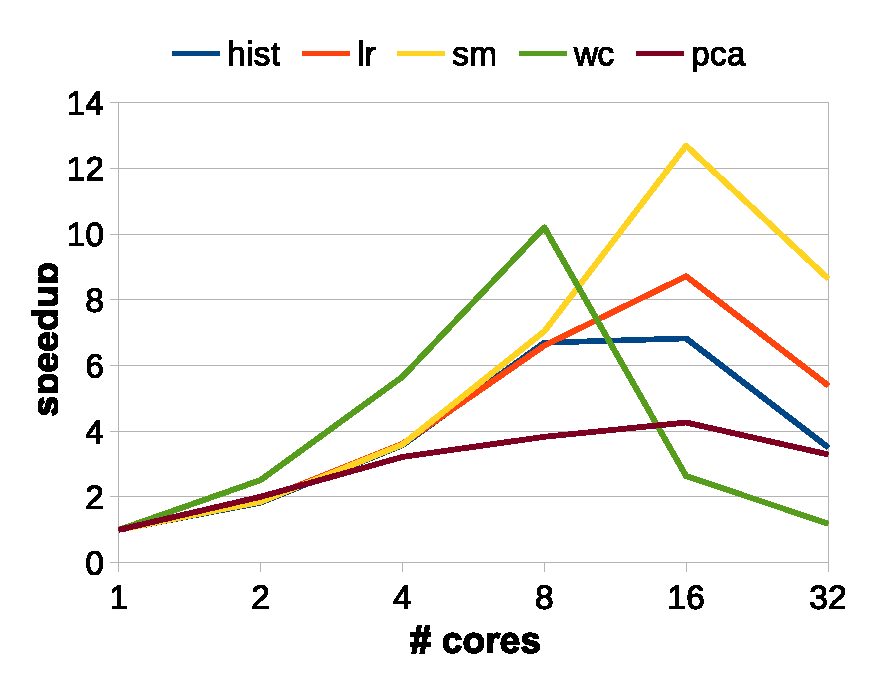
\includegraphics[width=0.45\textwidth]{eps/phoenix_speedup_jemalloc.eps}
%		\label{fig:phoenix:speedup:jemalloc}
%	}
%	\subfigure[\_\_tickect\_spin\_lock execution time percent of Phoenix-jemalloc]{
%		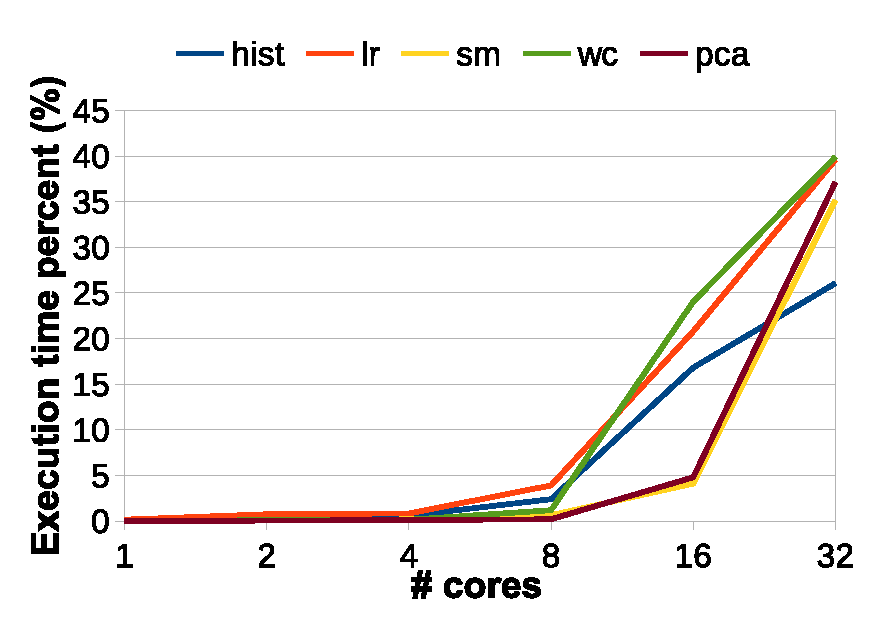
\includegraphics[width=0.45\textwidth]{eps/phoenix_spinlock_jemalloc.eps}
%		\label{fig:phoenix:spinlock:jemalloc}
%	}
%	\caption{scalability of Phoenix-jemalloc}
%	\label{fig:phoenix:scalability}
%\end{figure}
As the number of cores increase (from 1 to 8), the performance of Phoenix increase for all cases, i.e., the execution time decreasing. 
While For 16 to 32 cores, Phoenix performance keep decreasing with the increase of the number of cores.
\begin{figure}[!h!t]  
	\centering
	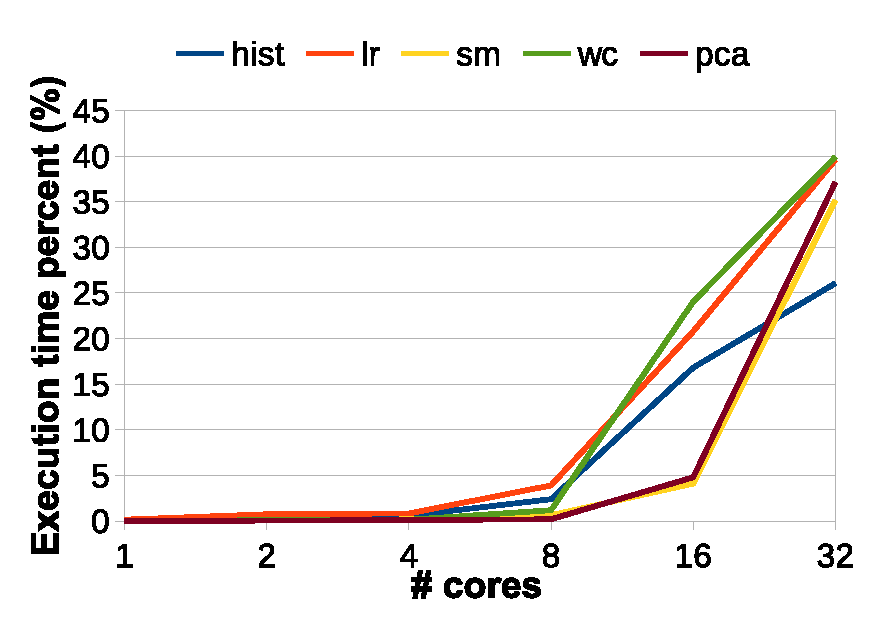
\includegraphics[width=0.45\textwidth]{eps/phoenix_spinlock_jemalloc.eps}
	\caption{speedup of Phoenix-jemalloc}
	\label{fig:phoenix:spinlock:jemalloc}
\end{figure}
At the same time, we collect \_\_ticket\_spin\_lock execution time percent by Linux perf to peek the contention in Linux kernal.
The result shows in Figure\ref{fig:phoenix:spinlock:jemalloc}.
We note serious contending lock takes place when increase the number of cores over 8 and as a result execution time will be drastically increased.
%When the number of dependent processes increases above the
%number of cores, serious contending lock takes place,
%and as a result execution time will be drastically increased.
%As the number of threads increases from 32 to 33, 
%there is a significant increase in execution time owing to .

At low cores, increasing .. resulted in speedup.
However, as more cores were added, the benefit was reversed due to the increased time spent in ticket\_spin\_lock. 

%通过使用sthread,我们能够提升scalability,降低tickect_spin_lock的开销,但是lr和hist两个应用程序的scalability比较差,将在section 5.4分析原因
%\begin{figure}[htpb]
%	\centering
%	\subfigure[speedup of \myds]{
%		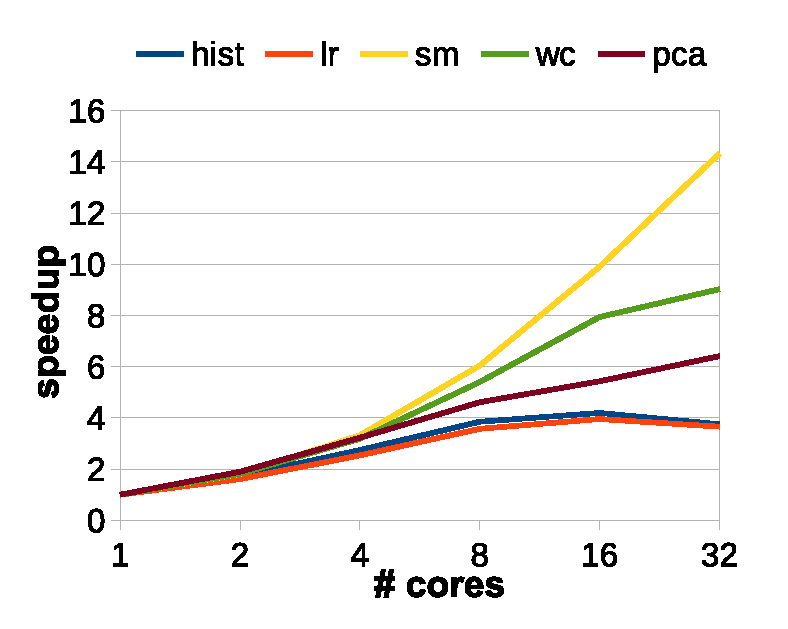
\includegraphics[width=0.45\textwidth]{eps/dmr_speedup.eps}
%		\label{fig:smr:speedup}
%	}
%	\subfigure[Execution time percent of \_\_tickect\_spin\_lock in \myds]{
%		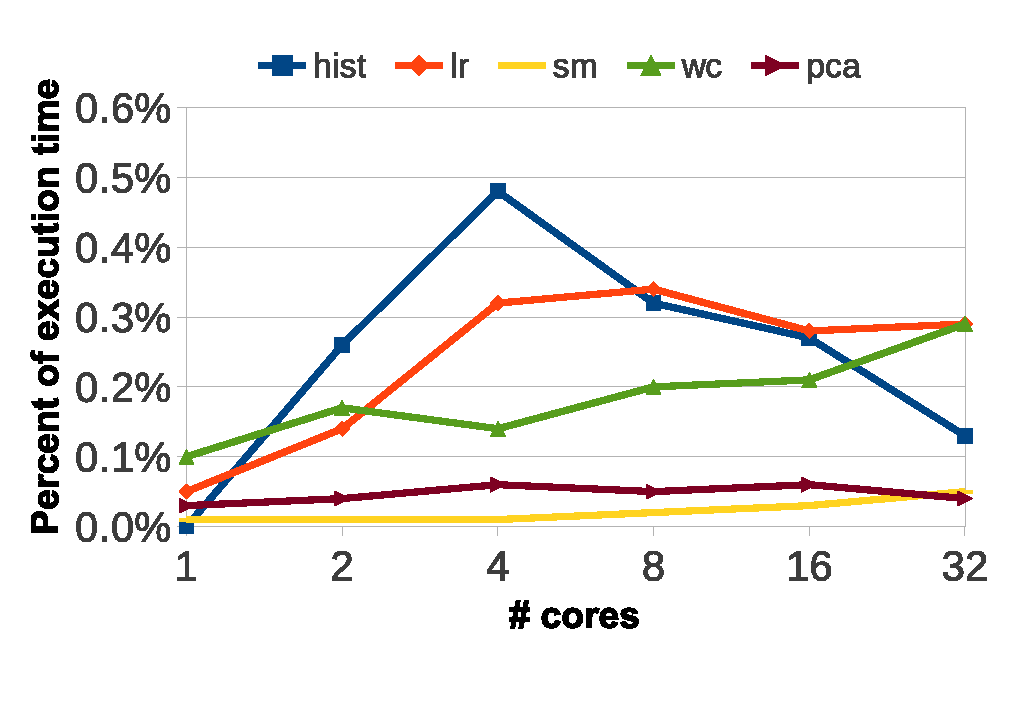
\includegraphics[width=0.45\textwidth]{eps/dmr_spinlock.eps}
%		\label{fig:smr:spinlock}
%	}
%	\caption{scalability of \myds}
%	\label{fig:smr:scalability}
%\end{figure}

Although with the scalable memory allocator, Phoenix can not scale up to 16cores.
 
\begin{figure}[!h!t]  
	\centering
	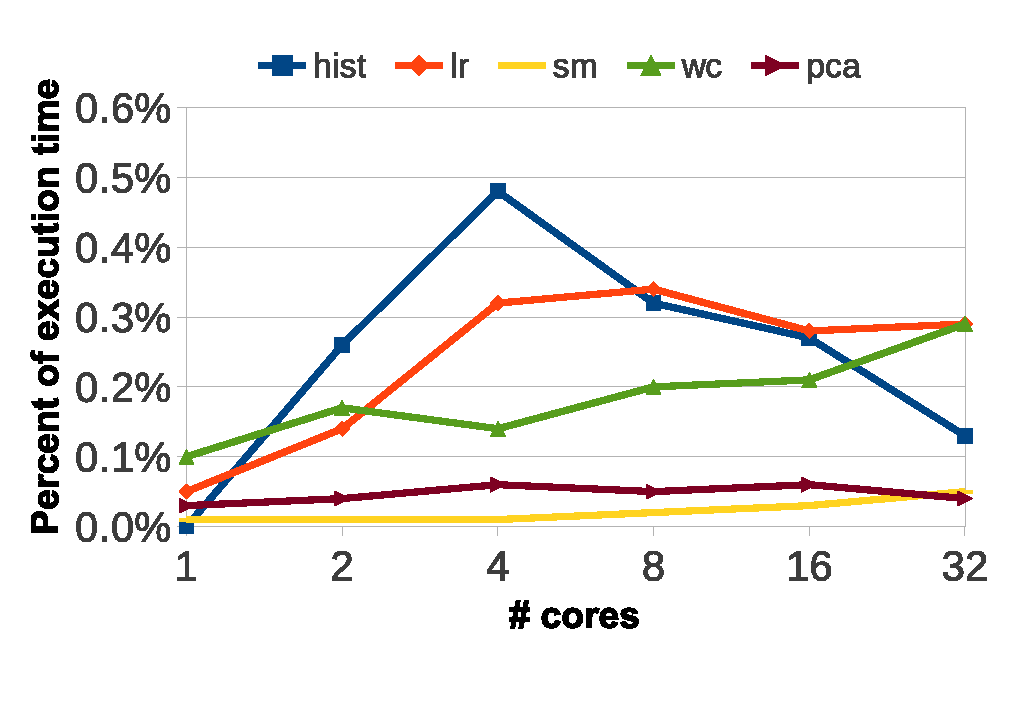
\includegraphics[width=0.45\textwidth]{eps/dmr_spinlock.eps}
	\caption{Execution time percent of \_\_tickect\_spin\_lock in \myds}
	\label{fig:smr:spinlock}
\end{figure}

Figure\ref{fig:smr:speedup} summarizes the scalability results for \myds.
Specially, workloads \codet{string\_match}, \codet{word\_count} and \codet{pca} scaled up to 32 cores.
And the performance of hist, wc, sm are scale linearly with the number of cores.
However, \codet{linear\_regression} and \codet{histgram} still did not scale particularly. 
We will discuss their bottlenecks in detail in subsection 5.4.
\begin{figure}[!h!t]  
	\centering
	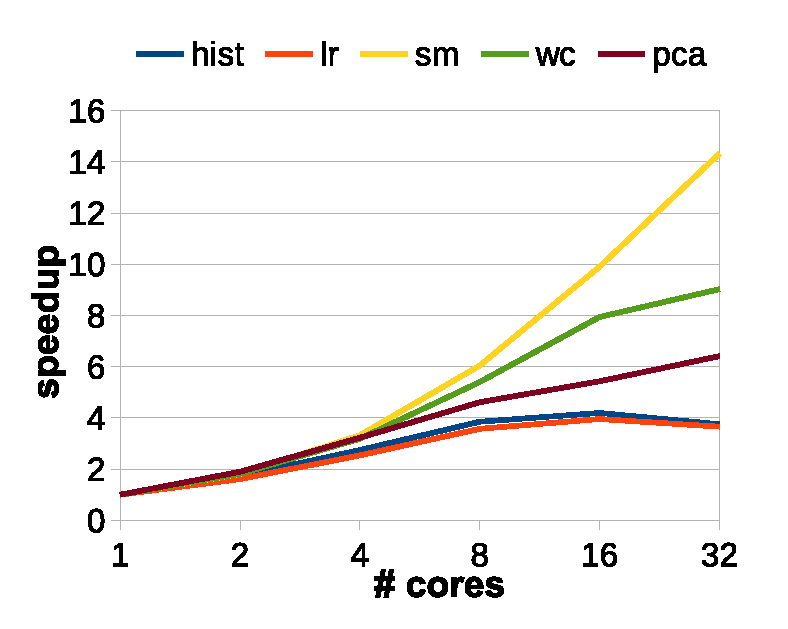
\includegraphics[width=0.45\textwidth]{eps/dmr_speedup.eps}
	\caption{speedup of Phoenix}
	\label{fig:smr:speedup}
\end{figure}

In our \myds, using \myth thread was sufficient to reduce the contention in Linux kernel. 
System Contention is evaluated using the execution time percent of \_\_ticket\_spin\_lock. 
Evaluation indicates (Figure\ref{fig:smr:spinlock}) that the locking overhead can be significantly reduced to less than 1\% of total runtime on 32 cores
%\begin{figure}[!h!t]  
%	\centering
%	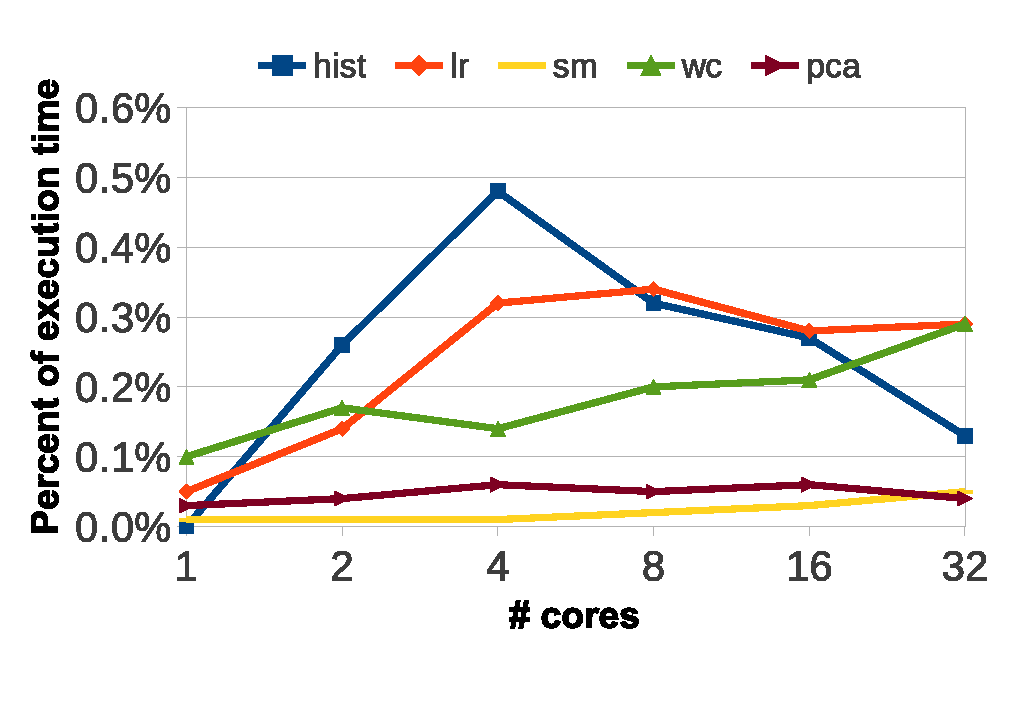
\includegraphics[width=0.45\textwidth]{eps/dmr_spinlock.eps}
%	\caption{tickect\_spin\_lock execution time percent of Phoenix}
%	\label{fig:smr:spinlock}
%\end{figure}

%We say a waiting thread is the thread which is waiting for shared
%data that produced by another thread. If using semaphore for
%synchronization, a waiting thread will be blocked and enlisted
%on the waiting queue by the OS scheduler. If using spinlock
%for synchronization, a waiting thread will do busy wait, i.e.
%spinning in a while loop. Embedded software applications
%that using semaphore to handle the synchronization could
%result in performance overkill, since it involves system calls
%translated into thousands of CPU instructions [1]; while using
%spinlock have problem of long busy-waiting time.

%When a running thread tries to read shared data,
%it must do busy wait until it has exhausted its time-slice
%or until another thread has withdrawn the occupation on the
%shared data. 




%System performance is evaluated using
%instructions per cycle (IPC). Higher IPC means
%better performance.
%Figure\ref{fig:perf:ipc} shows the IPC of Phoenix first increases 
%and then decreases as more threads are run on multi-core system.


To summarize, \myds demonstrated its performance and scalability for applications such as \codet{word\_count}, \codet{histgram} and \codet{pca}.
For applications such as \codet{linear\_regression}, \myds does not show its superiority, which we will analyze this result in detail in Section 5.4.

\subsection{ Impact of buffer Optimizations}
In Section 4.3, we discussed the organization of intermediate data is critical to the performance of many MapReduce applications.
Using the default hash buffer, need to gather the scatter key arrays together before sending them to the \codet{shared-channel}, which is time wasting.
we addressed this issue by providing a array implementation of buffer. 
Especially, array buffer, which is a continuous memory space, avoided buffer reallocation and coping.
However, not all the workloads benefited from the optimization.




%As described in Section 4.3, we provide two implementation of the local buffer in Map phase, i.e, hash buffer or array buffer.  
\begin{figure}[!h!t]  
	\centering
	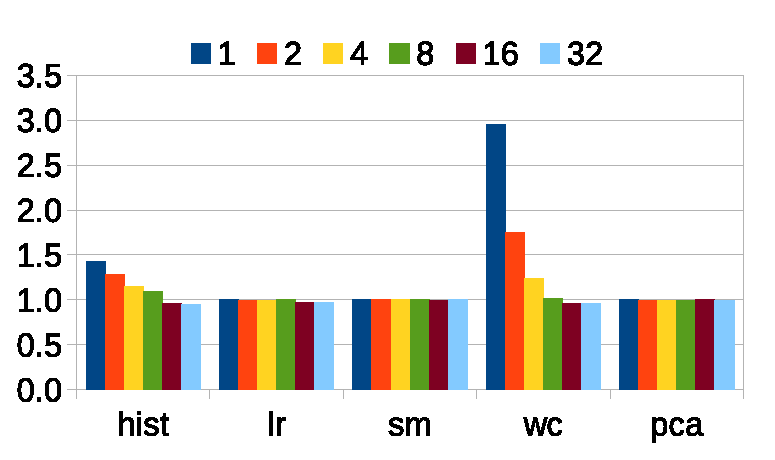
\includegraphics[width=0.45\textwidth]{eps/smr_diff_buffer.eps}
	\caption{the diffrent implementation of buffer}
	\label{fig:smr:diff:buffer}
\end{figure}

%As the number of threads increases (from 1 to 8), the
%execution times for both Pthread/C and MPI programs decrease
%for both workstation and supercomputer. For 9 threads to 32
%threads, Pthread/C and MPI execution times changes slightly
%on workstation. However for 9 threads to 32 threads, both
%Pthread/C and MPI execution times keep decreasing (in most
%cases) with the increase in number of threads on the
%supercomputer node. This is because we use 8 cores in the
%workstation while we use 32 cores in the supercomputer node.
%Execution time for large number of threads (9 to 33 and
%beyond) remains almost the same for the workstation because
%of no communication overhead. Results (see Figure 4) also
%show that MPI execution time on supercomputer increases
%significantly when the number of threads is increased from 32
%to 33 and beyond; but Pthread/C execution time on
%supercomputer remains almost unchanged. This is due to the
%communication overhead among the cores (32 cores in a
%supercomputer node) when using MPI message passing.
Figure\ref{fig:smr:diff:buffer} shows the 
From the Figure, it can be seen that although cases such as \codet{word\_count} and \codet{histgram} used array buffer has better performance, other benchmarks, e.g., \codet{linear\_regression}, \codet{string\_match} and \codet{pca}, did not.
So, for workloads that did generate a large number of key-value pairs, gather operation in hash buffer waster more time, as a result, array buffer will be better.

From the experimental results, it is observed that benchmarks yield better performance using \myds than Phoenix (in most cases). 
\myds has the advantage over Phoenix for pipelining map and reduce phases and separating address space by using \myth thread instead of shared memory Pthread. 
The performance of the \codet{histgram} implementation on Phoenix is the best, 30\%-95\%x better than the Phoenix implementation on the our 32-cores system.

\subsection{ Challenges and Limitations}
Although we were able to significantly improve the scalability of \myds, 
workloads \codet{histogram}, \codet{linear\_regression} still did not scale up to 32cores (as shown in Figure\ref{fig:smr:speedup}). 
%We used /usr/bin/time to assess where the execution time was
We collect each phase time information to find out where the execution time was being spent by using stub. 
The results denote that workloads on \myds waste more execution time in initialization phase, compared to Phoenix.
Figure\ref{fig:env:init} shows the initialization time of \myds and Phoenix.
Exactly, the initialized time of \myds is range 0.25s to 0.35s, while it is just about 0.001s in Phoenix.
\begin{figure}[!h!t]  
	\centering
	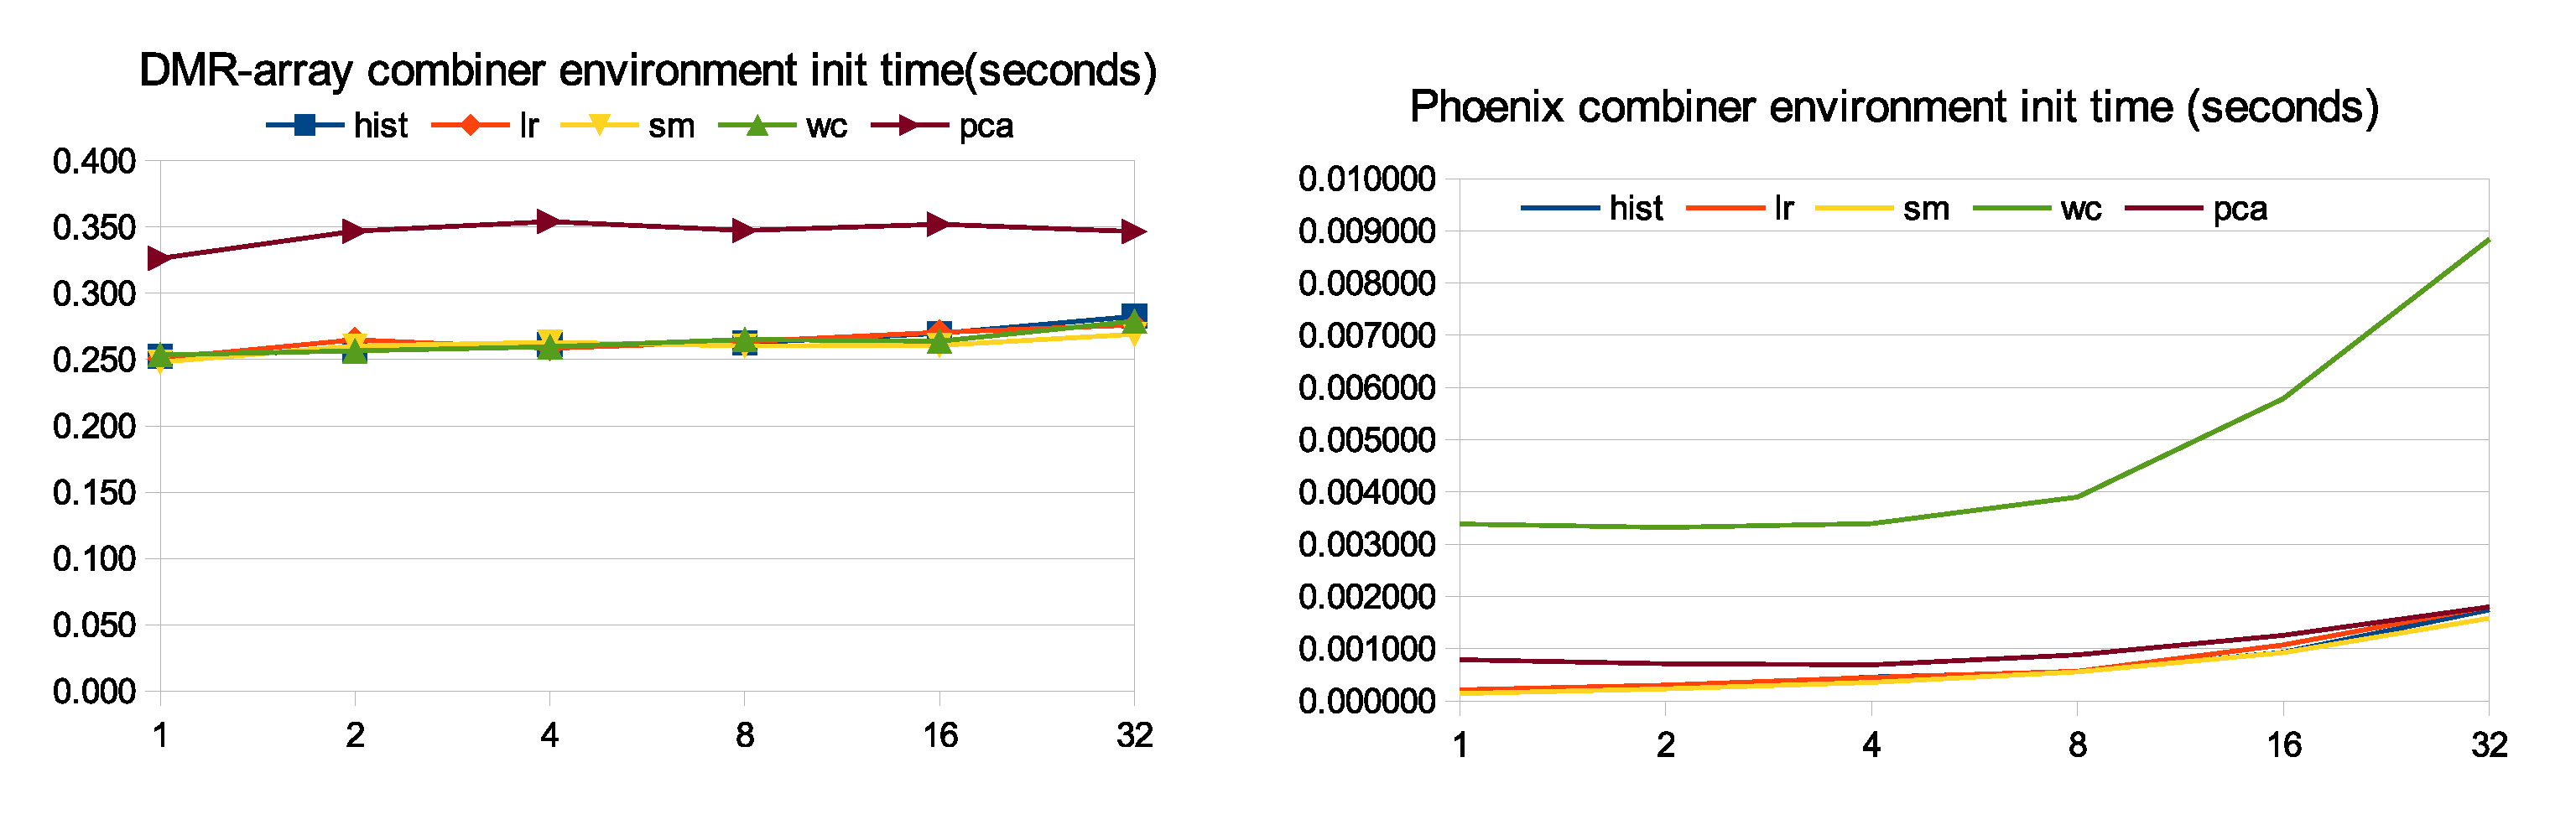
\includegraphics[width=0.5\textwidth]{eps/env_init.eps}
	\caption{initialization time of \myds and Phoenix}
	\label{fig:env:init}
\end{figure}


%解释为什么smr中的初始化时间会这么大
For multicore MapReduce library, most of initialized time is occupied in creating map and reduce threads.
Compared to thread in Phoenix, which based on Pthread, creating thread will spend more time in \myds because of more resource need to be allocated.
In addition, it will take more time for creating \codet{shared-channel} and setting up it.
From the experimental results (Figure\ref{fig:env:init}(b)), we observed that initialized time is small variation for different benchmarks and in different cores count, except for \codet{pca}.
Since there are two times mapreduce computation in \codet{pca}, which lead to two times initialization, it take more time than others benchmarks.
  

\begin{figure}[htpb]
	\centering
	\subfigure[Execution time and initialization time on histgram]{
		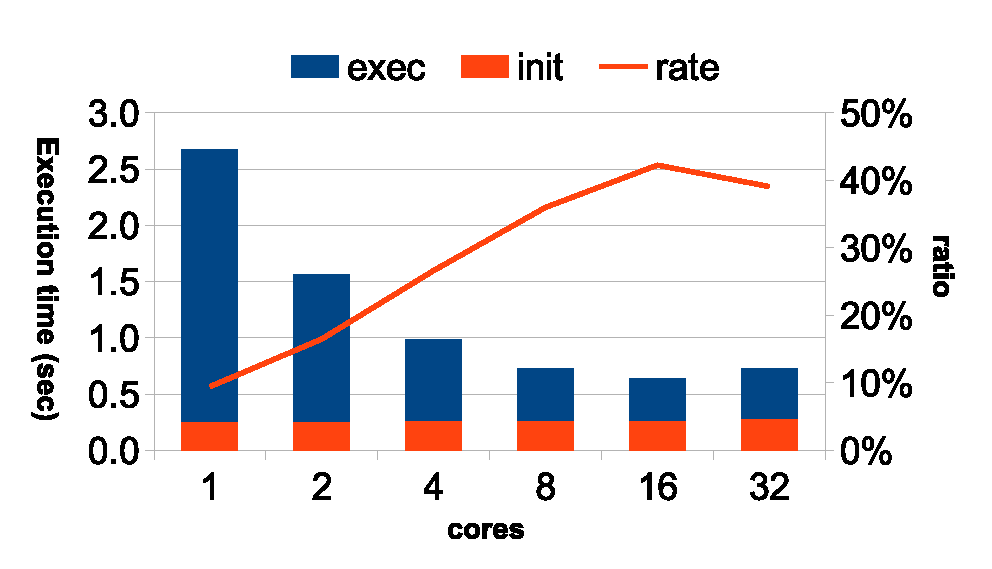
\includegraphics[width=0.45\textwidth]{eps/dmr_hist_init.eps}
		\label{fig:dmr:hist:init}
	}
	\subfigure[Execution time and initialization time on linear\_regression]{
		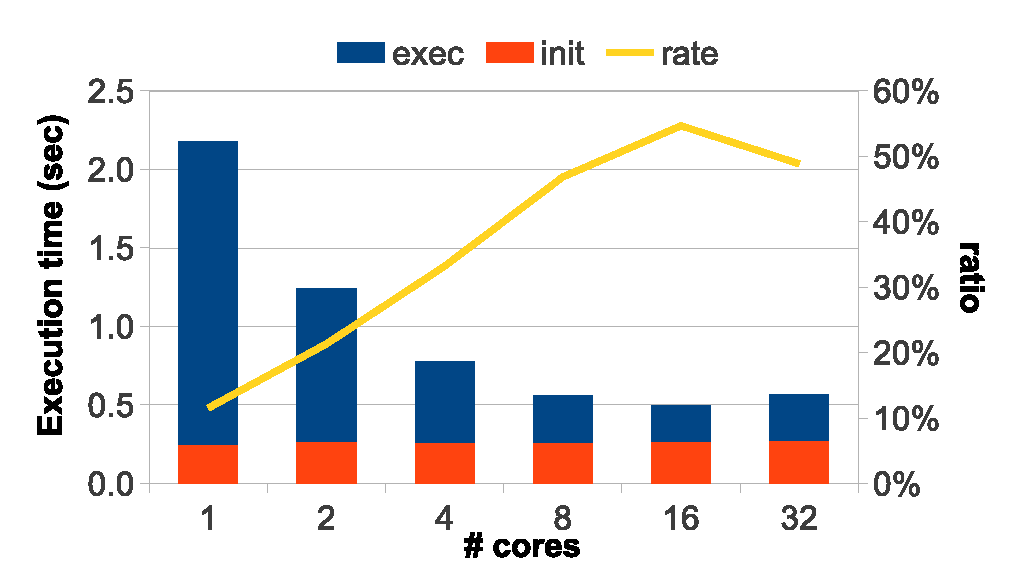
\includegraphics[width=0.45\textwidth]{eps/dmr_lr_init.eps}
		\label{fig:dmr:lr:init}
	}
	\caption{Initialize time with \myds}
	\label{fig:init}
\end{figure}


%这种较大较大的初始化对performance和scalability造成的影响


Figure \ref{fig:dmr:hist:init} shows the result with exec time defined as mapreduce actual execution time and init time as the initialization time before workers starting work. 
It was clear that the 2 non-scaling workloads shared two common trends. 
First, the total execution time of both \codet{histgram} and \codet{linear\_regression} less than 2.7s for all cores, which if far less than other benchmarks. 
Second, As the increasing number of cores, the portion of actual computation time (execution time) significantly decreased.
However, the initialization time is almost constant, which cause the init time ratio increase and dominate the total execution time at high cores count. 
As a result, the total execution time of \codet{linear\_regression} on Phoenix will less than on \myds.
%Second, the portion of actual computation time assumed by kernel code (sys /
%effective) significantly increased as we went beyond the single
%chip boundary.
%Second, both total execution time are short, While the portion of init time is 





